\documentclass[a4paper, oneside, 10pt]{book}

\usepackage{fancyhdr,verbatim, listings, color} 
\usepackage{shorttoc}
\usepackage[french]{minitoc}
\usepackage[pdftex]{graphicx} 
\usepackage[utf8]{inputenc}
\usepackage[T1]{fontenc}
\usepackage[frenchb]{babel}
\usepackage{amsmath,amssymb,mathrsfs}
\usepackage[french]{varioref}
\usepackage{url}
\usepackage{../nota}
\usepackage{../citation}
%\usepackage{../sommaire}

\graphicspath{%
  {../imgs/}%
  {imgs/}
}

% NOTES
\setlength{\largeurnota}{.8cm}
\newenvironment{attention}{%
  \begin{pictonote}{attention}}{\end{pictonote}}
\newenvironment{note}{%
  \begin{pictonote}{note}}{\end{pictonote}}
\newenvironment{question}{%
  \begin{pictonote}{question}}{\end{pictonote}}

\usepackage[pdftex=true,
    bookmarks         = true,
    bookmarksnumbered = true,
    bookmarks = true, 
    pdfstartview      = FitH,
    bookmarksopen     = true, 
    bookmarksopenlevel = 1, 
    hyperindex        = true,
    colorlinks        = true,
    %urlcolor          = red,
    %pdfborder         = {0 0 0}
    ]{hyperref}

\definecolor{colKeys}{rgb}{0,0,1} 
\definecolor{colIdentifier}{rgb}{0,0,0} 
\definecolor{colComments}{rgb}{0,0.5,1} 
\definecolor{colString}{rgb}{0.6,0.1,0.1} 

\lstset{
float=hbp,
basicstyle=\ttfamily\small,
identifierstyle=\color{colIdentifier},
keywordstyle=\color{colKeys},
stringstyle=\color{colString},
commentstyle=\color{colComments},
language=c++,
columns=flexible,
tabsize=2,
frame=trBL,
frameround=tttt,
extendedchars=true,
showspaces=false,
showstringspaces=false,
numbers=left,
numberstyle=\tiny,
breaklines=true,
breakautoindent=true,
captionpos=b,
commentstyle=\textit
}

\lstnewenvironment{cpp}{\lstset{language=c++}}{}

%% Define a new 'leo' style for the package that will use a smaller font.
\makeatletter
\def\url@leostyle{%
  \@ifundefined{selectfont}{\def\UrlFont{\sf}}{\def\UrlFont{\small\ttfamily}}}
\makeatother
%% Now actually use the newly defined style.
\urlstyle{leo}

\pagestyle{fancy} 



\hypersetup{
    pdfauthor   = {Clément Badiola, Samuel Da Silva},% 
    pdftitle    = {AL - Rapport de projet},%
    pdfsubject  = {Rapport de projet},% 
    pdfkeywords = {},% 
    pdfcreator  = {PDFLaTeX},% 
    pdfproducer = {PDFLaTeX}} 

\author{Clément~\textsc{Badiola} \and Samuel~\textsc{Da~Silva} \and \\
  Chargé de TD : David~\textsc{Auber}}
\title{Architecture logicielle \\ Rapport de projet}
\date{21 novembre 2012}

\begin{document}

\fancyhf{} 
\renewcommand{\chaptermark}[1]{\markboth{#1}{}} 
\renewcommand{\sectionmark}[1]{\markright{\thesection\ #1}} 
\fancyhead[R]{\bfseries\thepage}% Left Even, Right Odd - No de page 
\fancyhead[L]{\bfseries\rightmark} % Left Odd - Titre section 
\renewcommand{\headrulewidth}{0.5pt}% filet en haut de page 
\addtolength{\headheight}{0.5pt} % espace pour le filet 
\renewcommand{\footrulewidth}{0pt} % pas de filet en bas 
\fancypagestyle{plain}{ % pages de tetes de chapitre 
  \fancyhead{} % supprime l’entete 
  \renewcommand{\headrulewidth}{0pt} % et le filet 
}

\fancypagestyle{plain}{
	\fancyhf{}
	\fancyfoot[C]{\thepage}
	\renewcommand{\headrulewidth}{0pt}
	\renewcommand{\footrulewidth}{0pt}}

\dominitoc

\maketitle

\frontmatter

\chapter{Introduction}

Ce document est le rapport d'un projet d'architecture logicielle effectué par un binôme d'étudiants dans le cadre de leur deuxième année de Master.

Le projet concerne la modélisation des données d'un jeu de type \emph{RTS} (Real-Time Strategy). Il s'agissait de développer des fonctionnalités en utilisant nos connaissances des patterns et des bonnes pratiques en terme de génie logiciel.

\vfill

\textbf{Mots-clés :} architecture logiciel, pattern, conception, refactoring

\vfill
 %Contexte, problematiques à étudier.

\tableofcontents

\mainmatter

\chapter{Cahier des charges}
\minitoc

Comme nous venons de le voir, notre projet consiste à nous intéresser à la modélisation des données associées à un jeu de type \emph{RTS} . Définissons donc pour ce programme les objectifs du point de vue non-fonctionnel.

\section{Besoins non-fonctionnels}

\subsection{Refactoring}\label{refactoring} 

Le refactoring consiste à retravailler un code source dans le but d'améliorer sa lisibilité et son efficacité, et de simplifier sa maintenance.
L'introduction de nouveaux patterns induit le besoin de refactoriser souvent le code afin de simplifier
le codage et la compréhension.
En plus d'un simple nettoyage, cela nous amène à vérifier que notre architecture répond toujours aux
objectifs fixés.

L'objectif est bien sûr d'obtenir un gain de clarté, de lisibilité, de maintenabilité, et probablement de performances. Nous pouvons ainsi continuer l'ajout de fonctions sur une base saine.

\subsection{Transparence pour le client}

Nous pensons qu'un des objectifs du génie logiciel est de tenter d'obtenir une architecture telle que l'apport
de nouvelles fonctionnalités se fasse de manière transparente pour le client. Nous pourrions donc ajouter des
contraintes ou des fonctions sans que le \emph{main} ou les tests unitaires soient dégradés.

\subsection{Flexibilité}

La flexibilité d'une architecture est une pierre angulaire pour la maintenabilité d'une application.
Dans cette optique, nous devons garder notre code le plus simple possible, mais également penser aux contraintes
induites par l'utilisation des patterns.
 %Présentation des fonctionnalités demandées.
\chapter{Architecture}
\minitoc

L'architecture constitue un des éléments les plus importants pour le développement d'une bonne application.
Voici les concepts sur lesquels nous nous appuyons pour réaliser une architecture cohérente :  

\begin{itemize}
  \item Garder une architecture la plus simple possible. Chaque classe représente quelque chose de précis.
  \item Ranger les méthodes dans les bonnes classes.
  \item Limiter les attributs des classes afin de limiter les bugs.
  \item Limiter les dépendances externes et au langage. Les langages évoluent vite et il peut être parfois intéressant de pouvoir passer une application sur un autre langage.
\end{itemize}

\section{Diagramme des cas d'utilisation}

Nous avons réalisé un schéma des cas d'utilisations, visible en figure \vref{usecase} afin de synthétiser les besoins de l'utilisateur, pour offrir une vision simplifiée du système. Nous rappellerons brièvement les fonctionnalités par la suite.

\begin{figure}[h]
\begin{center}
    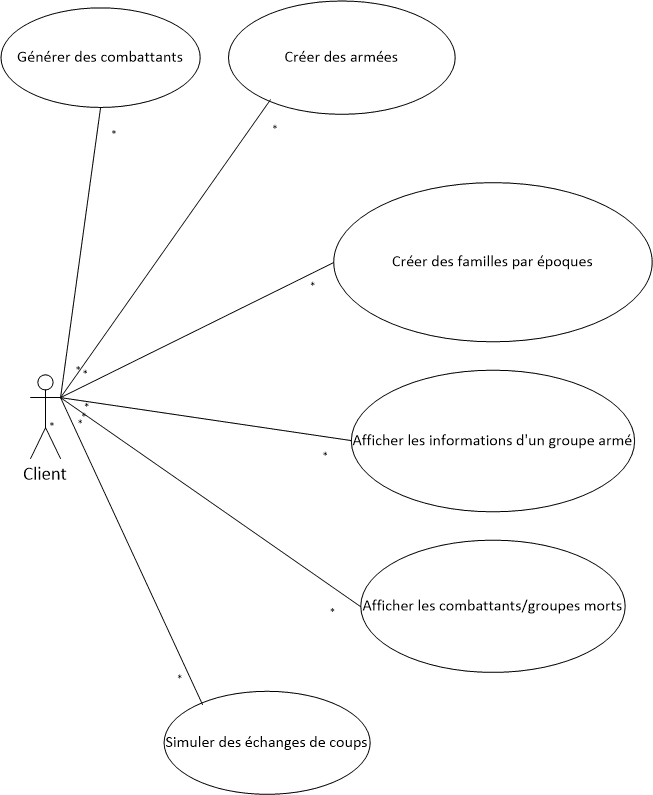
\includegraphics[width=12cm]{diagramme-usecase}
\end{center}
    \caption{Diagramme de cas d'utilisation}
    \label{usecase}                      
\end{figure}

\subsubsection{Générer des combattants}

Le client peut générer un combattant d'une classe spécifique. Il génère un combattant en utilisant un des types disponibles. Il doit spécifier l'armement du combattant après l'avoir généré.

\subsubsection{Simuler des échanges de coups}

Si des combattants ont été auparavant générés, ils peuvent s'échanger des coups, qu'ils soient équipés ou non.
Un combattant pourra frapper une cible ou parer un coups.

\subsubsection{Créer des armées}

Les armées sont composées d'éléments qui peuvent être des groupes de combattants ou des combattants. Les armées
peuvent frapper une cible ou parer une attaque.

\subsubsection{Afficher les informations d'un groupe armé}

Le client peut afficher les combattants d'un groupe armé ou compter les effectifs d'un groupe armé.

\subsubsection{Afficher les combattants morts et les groupes décimés}

Le client peut être averti du décès d'un combattant ou de l'éradication d'un groupe armé. Il peut prévenir les
amis d'un combattant du décès de celui-ci. Il peut aussi être averti du nombre de morts au fur et à mesure de
l'évolution des combats.

\subsubsection{Créer des familles de combattants par époques historiques}

Le client peut créer des combattants spécifiques à une époque et les équiper avec le type d'armement conforme
à cette époque. Par exemple, un guerrier Cromagnon ne se verra pas équipé d'une armure Terminator.
\section{Les classes}

Le diagramme global des classes de l'architecture a été réalisé à l'aide du logiciel \emph{Architexa} intégré à \emph{Eclipse}. Nous ne parlerons que de notre architecture finale, obtenue au fur et à mesure du refactoring.

Étant donné l'étendue de l'application, nous ne pouvons pas présenter de diagramme UML à la fois complet et lisible dans ce rapport. Voici le diagramme des classes sans les méthodes, en figure \vref{classes-final}. En rouge la partie développeurs, en bleu le cœur de l'application (côté client), et en vert les classes plus utilitaires.

\begin{figure}[h]
\begin{center}
    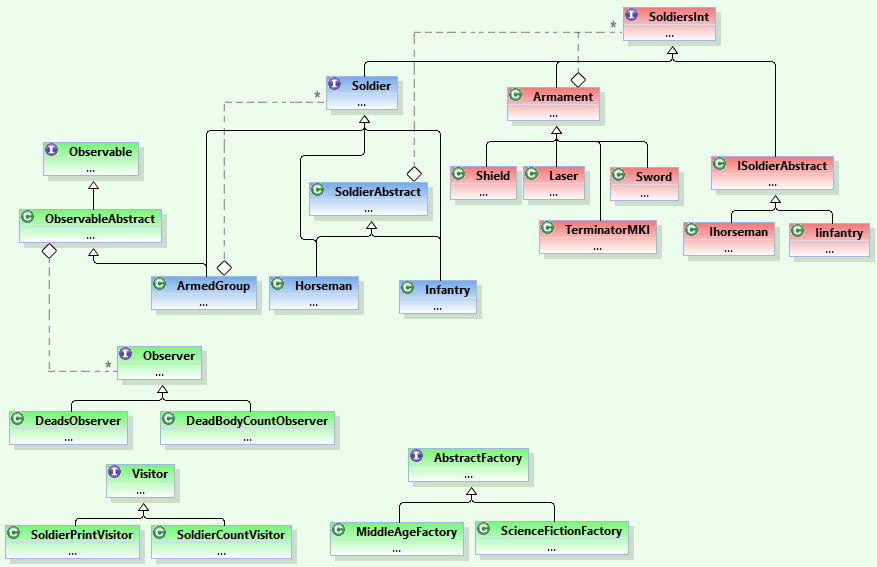
\includegraphics[width=11cm]{diagramme-classes-final}
\end{center}
    \caption{Diagramme de classes de l'application}
    \label{classes-final}
\end{figure}

 %Présentation cas d'utilisation, architecture générale
\chapter{Travail}
\minitoc

%Dans chaque section (pour chaque pattern) : 
%Un résumé de ce qu'est le pattern, à quel problème il répond.
%Puis un schéma d'architecture localisée sur ce pattern.
%Expliquer quelques diagrammes de séquence.
%Choix d'implémentation, avantages et inconvénients du pattern.
\section{Travail}
%travail_decorator
\subsection{Décorateur}
\begin{figure}[h]
\begin{center}
    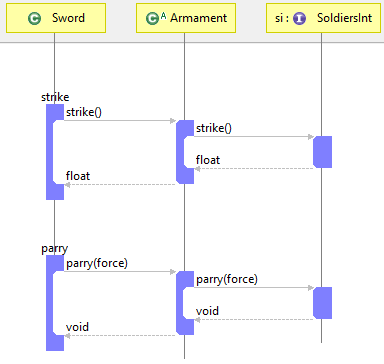
\includegraphics[width=11cm]{diagSeqDecorator}
\end{center}
    \caption{Diagramme de séquence du pattern décorateur}
    \label{sequence-decorateur}
\end{figure}

%travail_proxy
\subsection{Procurateur}
\begin{figure}[h]
\begin{center}
    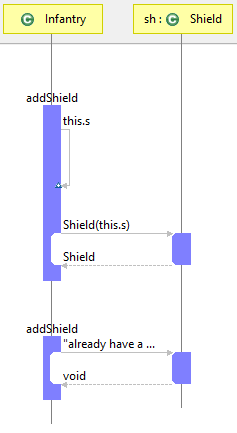
\includegraphics[width=11cm]{diagSeqProxy}
\end{center}
    \caption{Diagramme de séquence du pattern procurateur}
    \label{sequence-procurateur}
\end{figure}

%travail_composite
\subsection{Composite}
\begin{figure}[h]
\begin{center}
    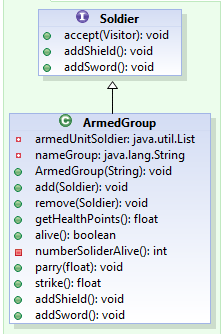
\includegraphics[width=11cm]{diagClassComposite}
\end{center}
    \caption{Diagramme de classes du pattern composite}
    \label{classes-composite}
\end{figure}

La seconde étape dans le projet consistait à rajouter la possibilité pour le client de créer des groupes armés. Un groupe armé de soldats peut être composé de plusieurs groupes armés, eux-mêmes décomposables en sous-groupes armés, et ainsi de suite. Cette notion de groupes armés fait ici apparaître une structure d'arbre avec des éléments composés d'autres éléments, structure qui fait penser à une hiérarchie. 
C'est pour cela que nous avons appliqué le pattern Composite, visible en figure \vref{classes-composite}, en créant une classe \emph{ArmedGroup} contenant une référence vers un objet \emph{Soldier} (qui représente notre \emph{procurateur}, ce que manipule le client).

%travail_visitor
\subsection{Visiteur}
\begin{figure}[h]
\begin{center}
    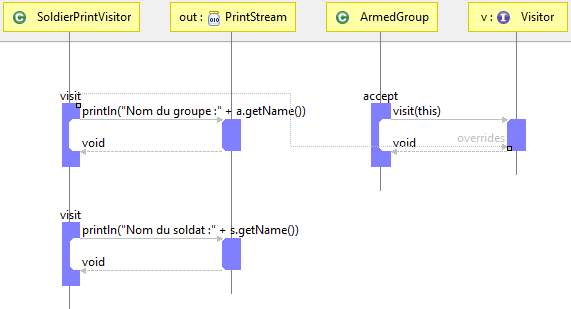
\includegraphics[width=11cm]{diagSeqVisitor}
\end{center}
    \caption{Diagramme de séquence du pattern visiteur}
    \label{sequence-visiteur}
\end{figure}

Nous avions à la fois des groupes armés ainsi que des soldats de différentes catégories. Afin de faciliter l'ajout de nouvelles fonctionnalités à la fois sur les groupes armés et sur les soldats, nous avons mis en place le pattern \emph{Visiteur}. Sans ce pattern, à chaque ajout de fonctionnalités, nous étions obligés de rajouter les méthodes dans nos classes \emph{Horseman}, \emph{Infantry} et \emph{ArmedGroup}, d'autant plus si nous voulions faire des traitement différents en fonction de chaque classe. Grâce au pattern \emph{Visiteur}, l'ajout de fonctionnalités supplémentaires (comme l'affichage de tous les soldats formant un groupe armé ou le comptage des effectifs de soldats par rapport à leur type au sein d’un groupe armé) se fait maintenant dans une seule classe, sans avoir à toucher le reste du code. Nous avons créé une classe \emph{SoldierPrintVisitor} pour ajouter la fonction d'affichage des soldats ainsi que la classe \emph{SoldierCountVisitor} pour ajouter la fonction de comptabilisation. Vous pouvez voir un exemple du déroulement des appels de méthodes en figure \vref{sequence-visiteur}. Tout ceci est totalement transparent vis-à-vis du reste du code : c'est là tout l'intérêt du pattern \emph{Visiteur}. On n'applique donc qu'un nombre minimal de modifications sur les autres classes de l'application et nous avons la possibilité de faire des traitements spécifiques pour chacune des classes de l'application. En résumé, nous pouvons maintenant ajouter des fonctionnalités sur les objets de notre choix sans toucher au reste du code.

%travail_observator
\subsection{Observateur}
\begin{figure}[h]
\begin{center}
    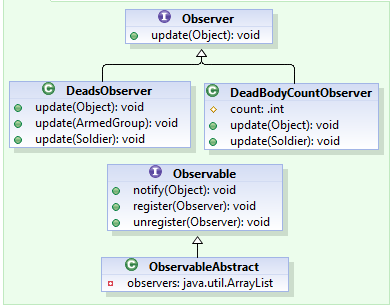
\includegraphics[width=11cm]{diagClassObserver}
\end{center}
    \caption{Diagramme de classes du pattern observeur}
    \label{classes-oberveur}
\end{figure}

Une des problématiques de ce projet était de pouvoir suivre le déroulement des conflits au fur et à mesure du déroulement de l’action. Nous aurions pu produire de nombreux print dans nos fonctions, ce qui aurait généré des affichages au fur et à mesure du déroulement des batailles. Cependant, cette méthode est peu flexible et peu maintenable ! 
C'est donc ici que le pattern \emph{Observateur} va être intéressant, car il nous permet d'observer un objet et d'être notifié de ses changements afin d'appliquer les traitements adéquats suite à ces changements. 
Ainsi, pour afficher au fur et à mesure les noms des soldats morts au sein d'un groupe armé ainsi que les armés détruites, nous avons mis en place le système visible en figure \vref{classes-oberveur}. Il est composé en premier lieu d'une interface \emph{Observer} avec pour sous-classe \emph{DeadsObserver}. Cette dernière se chargera de réaliser l'affichage. Nous avons également rendu observable notre classe \emph{ArmedGroup} en créant l'interface \emph{Observable}. \emph{ObservableAbstract} implémente cette interface et contient une liste d'\emph{Observers}, liste qui permet à l'objet, lorsqu'il change, d'en informer tous ses observateurs. 
Cette classe est également intéressante car elle permet de définir une interdépendance de type un à plusieurs, de tel façon que si on souhaite envoyer des télégrammes d’excuse à une liste d'ami une fois qu'un soldat meurt, on pourra notifier tous les objets qui dépendent du mort. L'inconvénient et la limite du pattern est que le graphe des relations d'observation peut vite devenir complexe. En effet, si l'on veut mettre en place le système des envois de télégrammes d’excuse à ses amis, c'est à dire à des soldats de l'armé, il va falloir que chaque objet soldat soit observé par tous les autres objets soldat « amis », ce qui implique la création de nombreux objet de type Observer (autant d'observer que de soldat) provoquant alors un ralentissement notable du programme ! Au vue de ces dernières remarques, nous n'avons pas retenu la fonction des télégramme via ce pattern là.

%travail_singleton
\subsection{Singleton}

%travail_abstract_factory
\subsection{Fabrique abstraite}
La dernière partie du projet consistait à créer plusieurs familles de soldats historiquement cohérentes, c'est à dire que pour une famille donnée, le type d'armement devait être conforme à son époque.

Pour le client, la notion d'époque vis à vis des armes doit rester transparente, en effet, on veut associer les bonnes armes au soldat construit par le client sans qu'il est à se soucier de la cohérence de son habillement, c'est à dire sans qu'il est à spécifier lui même les classes concrètes correspondant aux armes d'une époque ou d'une autre pour habiller son soldat. Ainsi donc, le client n'aura pas accès au processus de construction de son équipement (tel arme de défense pour telle époque, telle arme d'attaque pour telle époque), tout se fera automatiquement.

Pour réaliser cette demande, nous avons utilisé le pattern Fabrique abstraite. Nous avons donc créé une classe AbstractFactory comportant les méthodes setDefensiveWeapon(Soldier s) et setOffensiveWeapon(Soldier s) permettant d'affecter une arme défensive/offensive conforme à l'époque à un soldat donné. Ces méthodes se chargeront alors de la construction de l'équipement souhaité, en toute conformité avec l'époque. L'implémentation de ces deux méthodes se trouve dans les classes MiddleAgeFactory et ScienceFictionFactory, deux classes représentant deux époques différente. L'armement pourra donc être construit différemment en fonction de l'époque (par exemple les soldats de l'époque moderne seront équipés de laser).
Nous avons également rajouté des méthodes dans la fabrique permettant si besoin de construire des soldats de type différent.

Ainsi donc, grâce au pattern Fabrique abstraite nous pouvons garantir le maintient de la cohérence de nos équipements et de nos soldats en fonction de l'époque.
\section{Tests}

Afin de garantir la fiabilité de notre livrable, nous réalisons une série de tests unitaires et de tests fonctionnels. Les tests unitaires nous permettent de nous assurer du bon fonctionnement de certaines parties déterminées du logiciel. 

\subsection{Tests de la génération de combattants}
Nous réalisons un ensemble de génération de soldats tout en les équipant de pièces
d'armement puis nous vérifions la cohérence de leur force de frappe et de leur réaction
aux attaques adversaires.

\subsection{Tests de la génération de groupes armés}
Nous générons un ensembles de groupes composés de soldats puis nous vérifions que les groupes
sont bien cohérents par rapport aux combattants assignés.

\subsection{Tests des combats}
Nous faisons combattre des combattants et des groupes pour vérifier la cohérence de leurs réactions aux actions d'attaque et de défense.

\subsection{Tests des contraintes d'équipement}
Les combattants et groupes armés sont équipés d'une arme ou d'un bouclier puis ré-équipés d'un même type
d'armement pour vérifier qu'ils ne possèdent pas ensuite deux fois le même type d'équipement.

\subsection{Tests des observateurs}
Les observateurs doivent fournir un résultat prédéterminé pour des groupes armés ou des combattants sur
un scénario fixé. Nous vérifions que les résultats correspondent au scénario.

\subsection{Tests des fabriques}
Les fabriques doivent permettre de générer des combattants d'une époque particulière et d'équiper ces combattants
avec l'armement de l'époque. Nous testons que les combattants soient bien ceux attendus pour les époques du
moyen-age et du futur lointain. Nous testons également que leur équipement soit bien conforme à l'époque. Par
exemple, un \emph{Space marine} ne sera pas équipé d'une épée en bois, mais d'un laser.
 %Présentation de chaque pattern utilisé (le travail s'articule autour des patterns...)
\chapter{Bilan}
\minitoc

\section{Bilan}

En conclusion, nous pouvons dire que le bilan général est plutôt bon. Nous avons globalement satisfait les besoins client tout en réalisant nos objectifs initiaux en terme de refactoring et de qualité.

Au niveau de l'architecture, les méthodes sont restées simples, ce qui limite selon nous les sources de bugs. Nous limitons les dépendances avec les bibliothèques Java. L'application est donc plus maintenable et évolutive.

\subsection{Échecs}

Malgré ce bilan positif, nous déplorons le manque de temps pour mélanger l'utilisation intelligente des patterns et des principes de généricité et d'introspection, qui forment une combinaison pouvant répondre à certains problèmes liés à l'introduction de patterns.


\section{Si c'était à refaire…}

Si c'était à refaire, nous aborderions le problème différemment. En incluant nos connaissances en gestion de projets, nous pourrions aborder les problèmes liés à la complexification des phases d'intégration. En connaissant les patterns aux sein d'une équipe, nous aurions pu mesurer les effets de leur utilisation dans le cadre d'un projet utilisant les
méthodes agiles, comme l'\emph{XP} par exemple.

%\section{Perspectives}
%Voir si on met quelque chose dedans ou non.



\appendix
\backmatter
\listoffigures

%\tableofcontents

\newpage
\pagestyle{empty}

Rapport de projet d'architecture logicielle.\\
Wargame data modelizing.\\
Master 2, 2012

\vfill

Les sources de ce rapport sont disponibles librement sur \url{https://github.com/mr-nours/rapport-al}.

\end{document}
